\section{Applications in smart environments}
\label{ch:rel_se_app}
\begin{table}[htbp]
  \centering
  \caption{Application domains and relevant works}
    \begin{tabular}{rl}
    \toprule
    Application Domain & Relevant Works \\
    \midrule
    \multirow{4}[0]{*}{Indoor Localization} & Braun - AmbiTrack camera system \cite{braun2013ambitrack} \\
          & Chintalapudi - EZ Indoor localization \cite{ chintalapudi2010indoor} \\
          & Mulloni - signpost markers \cite{mulloni2009indoor} \\
          & Pirkl - resonant magnetic coupling \cite{pirkl2013resonant} \\ [1em]
    \multirow{4}[0]{*}{Gestural interaction} & Zimmerman - hand gesture \cite{zimmerman1987hand} \\
          & Wilson - XWand pointing interaction\cite{Wilson2003} \\
          & Majewski - visual feedback \cite{majewski2013providing} \\
          & Liu - uWave \cite{liu2009uwave} \\
          & Pu - WiSee \cite{pu2013whole} \\[1em]
    \multirow{4}[0]{*}{Physiological sensing} & Cowie - emotion recognition \cite{cowie2001emotion} \\
          & Khosrowabadi - EEG emotion \cite{khosrowabadi2010eeg} \\
          & Wöllmer - multimodal emotion recognition \cite{wollmer2010context} \\          
          & Hoque - MACH \cite{hoque2013mach} \\
          & Koelstra - DEAP database \cite{koelstra2012deap} \\[1em]
    \multirow{4}[0]{*}{Activity recognition} & Bao - user-annotated acceleration data \cite{Bao2004} \\
          & Bulling - electrooculography \cite{bulling2011eye} \\
          & Lasecki - real-time crowd labeling \cite{lasecki2013real} \\
          & Oreifej - Hon4D \cite{oreifej2013hon4d} \\[1em]
    \multirow{4}[0]{*}{Smart appliances} & Gellersen - MediaCups \cite{gellersen1999mediacup} \\
          & Yeo - StickEar \cite{yeo2013stickear} \\
          & Tsai - Smart Medication Dispenser \cite{tsai2011smart} \\
          & Dementyev - Bistable Display Tags \cite{dementyev2013wirelessly} \\[1em]
    \multirow{4}[0]{*}{Mobile devices} & Ballages - mobile devices in ubiquitous computing \cite{ballagas2006smart} \\
          & Dearman - Bluetone \cite{dearman2009bluetone} \\
          	& Vajk - TiltRacer \cite{vajk2007using} \\
          & Nazari Shirejini - PECo \cite{shirehjini2004novel} \\
          & Olsson - mobile augmented reality \cite{olsson2012user} \\[1em]
    \multirow{4}[0]{*}{Autonomous systems} & Coradeschi - symbiotic robotic systems \cite{coradeschi2006symbiotic} \\
          & Broxvall - PEIS ecology \cite{broxvall2006peis} \\
          & Arndt - robotic frameworks \cite{arndt2013performance} \\
          & Huijnen - companion robotics and smart homes \cite{huijnen2011maybe} \\
    \bottomrule
    \end{tabular}%
  \label{tab:rel_se_apps}%
\end{table}

The field of smart environments is not strictly and conclusively distinguished from other fields in technology. It is using influences from disciplines including electric engineering, behavioral psychology, computer science, or mechanical engineering. Accordingly, it is difficult to formally list or distinguish all applications that are relevant or have been tackled in previous work. Thus, I will refer to previous collections of surveys, books and state-of-the-art in the associated disciplines smart environments, ambient intelligence and ubiquitous computing to get an informed selection of relevant applications that have been, or could potentially be supported by capacitive proximity sensors. The chosen collections of applications are taken from different collections of work that have been released in the past few years. Cook et al. that presented a survey on recent developments in smart environments research in 2007 \cite{cook2007smart}. Augusto et al. edited a book on ambient intelligence in 2009, including chapters on various domains and applications. Another source is the book \emph{Ubiquitous Computing} by Poslad, released in 2011 \cite{poslad2011ubiquitous}. Additionally, I will take into account recent  conferences and journals that are active in this regard, such as CHI, UbiComp, Ambient Intelligent International, the Journal of Ambient Intelligence and Smart Environments, or the International Journal of Human-Computer Studies.

The selected areas-of-interest are collected in Table \ref{tab:rel_se_apps}. I will briefly introduce relevant work in those domains and outline existing links to capacitive sensing applications. 

\subsection{Indoor localization}
The domain of indoor localization has been briefly touched, when discussing the different sensing technologies used in smart environments in Section \ref{ch:rel_sensor_tech}. The reliable tracking and localization of multiple users is a major challenge in smart environments. It is a very important contextual information that can be used to adapt the behavior of the environment. Often basic motion sensors are used, e.g. if just a single person should be detected or if there is a single area of interest that should be covered. However, determining a more exact location or following multiple users requires more sophisticated systems. If a varying number of non-relevant actors are moving in the environment, e.g. pets, the challenge is additionally increased. Together with Tim Dutz, I participated in the EvAAL competition 2013 with AmbiTrack, reaching a second place \cite{braun2013ambitrack}. The system was based on a set of affordable off-the-shelf cameras connected to different processing nodes that employ an efficient tracking algorithm based on background subtraction, ray intersections and clustering methods \cite{Braun2013MarkerFree}. It also supports analyzing the coverage of areas where it is installed, as shown in Figure \ref{fig:rel_app_indoor}.

\begin{figure}[ht]
\centering
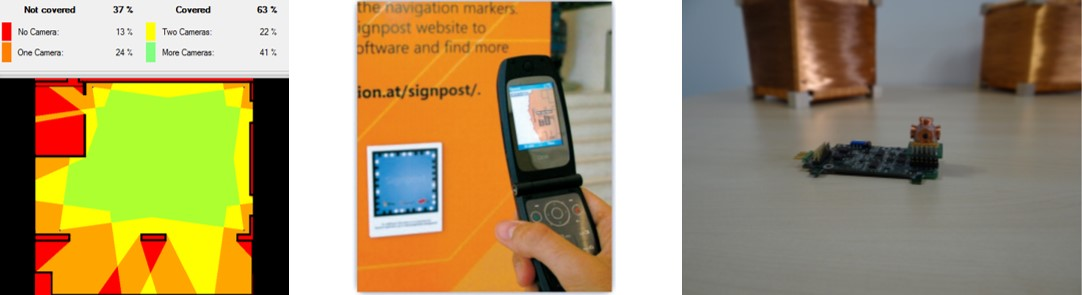
\includegraphics[width=0.8\textwidth]{images/rel_app_indoor}
\caption{\emph{Left:} Coverage of a room by camera fields of view - AmbiTrack \cite{Braun2013MarkerFree}. \emph{Middle:} Fiduciary marker photographed by camera phones \cite{mulloni2009indoor}. \emph{Right:} Magnetic coils in background and receiver circuit in foreground \cite{pirkl2013indoor}}
\label{fig:rel_app_indoor}
\end{figure}	

There are various indoor localization and tracking approaches that have been proposed in smart environments, including specific competitions that benchmark the different solutions against one another \cite{chessa_eval}. A common discrimination of localization systems is based on the type of object an actor has to wear in order to be successfully recognized. Active marker-based solutions require the person to carry a token that actively sends out signals. This is received by stations placed within the environment. Passive marker-based solutions require a token that is uniquely identifiable by external sensors, but is not sending any signal. Finally, there are marker-free solutions that do not require the actor to carry anything and instead rely on external sensors detecting unique features of the actor and following those within the environment. 

A common method is to use radiofrequency sensing, tracking a mobile token, e.g. based on 802.11 WiFi networks. A recent work in this domain has been presented by Chintalapudi et al. \cite{chintalapudi2010indoor}. Their EZ system relies on an existing WiFi infrastructure, the user carrying a mobile device with WiFi that also has periodic access to a GPS signal. It does not require any prior mapping or knowledge about the specific location or transmit power of the access points, but instead relies on a genetic algorithms to determine potential locations from a limited set of known locations and distances to access points calculated using the received signal strength (RSSI). 

Another system was presented by Mulloni et al. \cite{mulloni2009indoor}. They are using a set of fiduciary markers that are placed on signposts and can be photographed with smartphones. Based on an integrated mapping application the software will provide navigation from the current signpost to the desired destination. Thus, this is an example for an indoor localization system that relies on external markers, requires the user to wear a token in form of a smartphone and active user participation when the markers are photographed. The setup is shown in Figure \ref{fig:rel_app_indoor} in the middle.

A final example is a system created by Pirkl and Lukowicz based on resonant magnetic coupling \cite{pirkl2013resonant}. Using the magnetic field created by static coils, an arbitrary number of mobile receivers can localize themselves by measuring the field strength and estimating the distance from the different static coils. The system can be calibrated to ignore other magnetic objects in vicinity and enables a planar localization of about $1 m^2$ accuracy. The static coils can be seen in Figure \ref{fig:rel_app_indoor} in the background with the receiver circuit in the foreground.

\subsection{Gestural interaction}
Gesture recognition enables the detection of meaningful expressions of motion by a human body, including the hands, arms, face, head and body \cite{mitra2007gesture}. If these expressions are translated into machine commands the result is gestural interaction. The most expressive and explicit form of gestures are performed by the hands, further distinguished into free-air gestures and touch gestures that typically involve one or more fingers interacting with a surface. The second variety is called multi-touch.

\begin{figure}[ht]
\centering
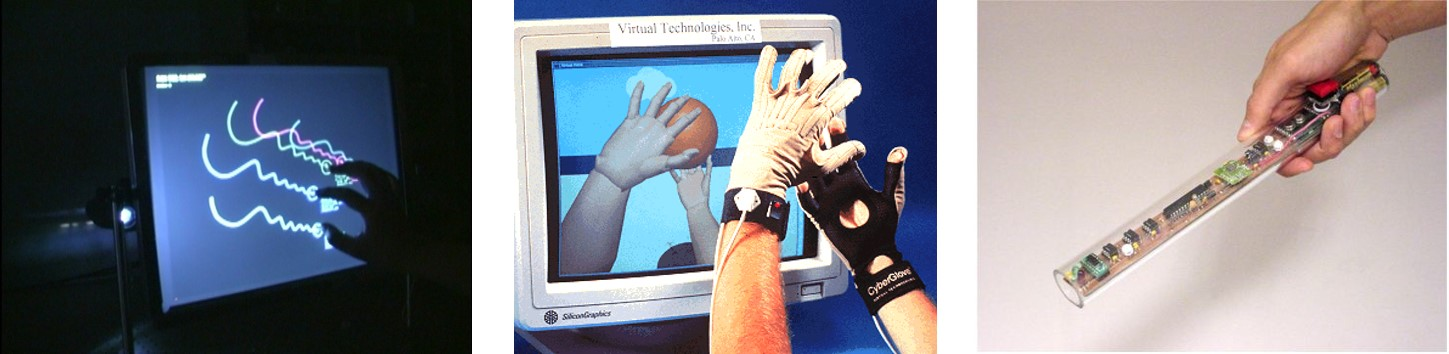
\includegraphics[width=0.8\textwidth]{images/rel_app_gesture}
\caption{\emph{Left:} FTIR multitouch table \cite{Han2005}. \emph{Middle:} DataGlove hand gesture system \cite{zimmerman1987hand}. \emph{Right:} XWand interaction device \cite{Wilson2003}}
\label{fig:rel_app_gesture}
\end{figure}

Jeff Han showed a low-cost system based on frustrated total internal reflection (FTIR) of infrared light. This system allows tracking ten or more objects in real-time on large surface areas \cite{Han2005}, as shown in Figure \ref{fig:rel_app_gesture} on the left. Acoustic systems are another popular technology in this domain. Surface acoustic wave (SAW) uses the signal decrease of ultrasonic waves as they pass through an object touching the surface to infer its location \cite{Armstrong1998}.
  
Throughout the years there have been various attempts to enable the tracking of gestures in free air. A common attempt in the late 1980s were data gloves, sensor-augmented gloves put on the hand that translated finger movements to gestural input, e.g. the system presented by Zimmerman\cite{zimmerman1987hand}. It uses optical sensors to measure the flex of the fingers and ultrasonic sensors to detect the absolute position and orientation of the hand. It is shown in Figure \ref{fig:rel_app_gesture} in the middle. Applications included the evaluation of hand impairments and object manipulations in three-dimensional scenes.

A different approach is performing gestural interaction supported by interaction devices that can sense orientation and position in the room. A popular example is the Nintendo Wii Remote that is used in gaming applications. A predecessor was the XWand by Wilson et al. \cite{Wilson2003}. This interaction device is using accelerometers to sense orientation and has infrared diodes that are tracked by an external camera system to determine the absolute position in the room. It is shown in Figure \ref{fig:rel_app_gesture} on the right. Using knowledge about the location of different appliances within this room, it is possible to control them by pointing in this direction. They later extended the system with a pointing device based on a laser that indicated the position in the environment currently pointed at \cite{Wilson2003a}. We have used a similar method, based on skeleton tracking provided by a Kinect and different varieties of pointing gestures \cite{majewski2013providing}.

An extension of accelerometer-based gesture systems was presented by Lui et al. \cite{liu2009uwave}. Their uWave system is capable of building a personalized gesture set using dynamic time warping and HMM classification, enabling a high recognition rate of almost $99\%$ using just one training sample. Additional applications of this approach include using personal gestures for authentication, reaching an error rate of approximately $3\%$. However, this method can be bypassed if the movements are observed and mimicked and thus is not suitable for critical applications.

I previously introduced WiSee presented by Pu et al. \cite{pu2013whole}. Using two sources of wireless signals, they are using the Doppler shift caused by the human body moving in the area and reflecting the signal to determine gestures. The system was able to detect nine different full-body gestures with a precision of $94\%$. The system uses the MIMO capabilities of modern WiFi systems to distinguish users and providing the option to support multiple users within an environment.

\subsection{Physiological sensing}
In the 1990s researchers began to distinguish different channels when interacting with machines. The explicit channel, whereas the user gives distinct commands to the user, and the implicit channel that comprises information about the user himself \cite{cowie2001emotion}. One interesting parameter to consider for this implicit interaction is emotion. Based on physiological cues it is possible to determine the current state of the user and translate it to an input for machines. Thus, an area has emerged that uses acquired physiological signals of the users to provide additional input. In this section I will present four different works of recent years that proposed important technologies and methods.

\begin{figure}[ht]
\centering
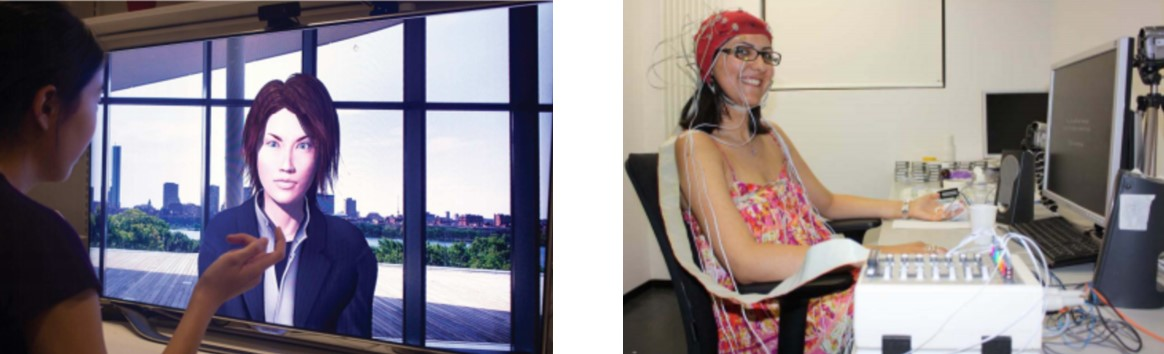
\includegraphics[width=0.8\textwidth]{images/rel_app_emotion}
\caption{\emph{Left:} MACH conversation coach system \cite{hoque2013mach}. \emph{Right:} Study setup to collect emotion data \cite{koelstra2012deap}}
\label{fig:rel_app_emotion}
\end{figure}

Khosrowabadi et al. presented a machine learning approach to discriminate four different emotions from EEG readings \cite{khosrowabadi2010eeg}. The subjects were asked to fill out self-assessment questionnaires regarding their emotional state with the states being induced by a set of pictures. The signals were classified using a self-organizing map and nearest-neighbor classification. The system was able to correctly classify $84.5\%$ of four different emotional states.

A multimodal emotion recognition system based on speech and facial expression was introduced by Wöllmer et al.  \cite{wollmer2010context}. They apply a method based on long short-term memory networks that allows to model long-range temporal dependencies between features. They combine 46 facial markers and a variety of waveform speech features that are combined using a correlation-based feature subset selection that leads to a selection between 66 and 224 features. They are able to improve the recognition performance compared to HMM-based classifiers by $4\%$.

An example application for emotion-aware systems has been presented by Hoque et al. \cite{hoque2013mach}. \emph{MACH: My Automated Conversation coacH} is a training system that tries to improve the social skills of its users. It collects facial expressions, speech data and analysis prosody from an attached camera to create a personalized feedback of the users behavior when talking to a virtual agent. This agent is shown in Figure \ref{fig:rel_app_emotion} on the left. A study with 90 participants showed a significant performance improvement as opposed to the control group. 

In this domain it is also very important to build databases of labeled emotions and physiological signals that allows other researchers to try new methods. Koelstra et al. \cite{koelstra2012deap} created a database by collecting EEG information, playing different video clips and collecting the perceived emotions in a self-assessment. This database includes the physiological signals of 32 users and frontal face videos of 22 users that are reacting to 40 different videos. The setup of this study can be seen in Figure \ref{fig:rel_app_emotion} on the right.

\subsection{Activity recognition}
Activity recognition, also called situation awareness, describes the interpretation of sensor data into higher domain-level information that relates to the given situation \cite{ye2012situation}. To give an example, a single temperature reading of $15\,^{\circ}{\rm C}$ can be combined with the information that the sensor is in the sleeping room, the time is $21:00$ and we know that the inhabitant of the environment is typically going to sleep at $22:00$. In this case we can infer the activity \emph{user will go to bed soon} and trigger the action \emph{heat up sleeping room}. There is a plethora of different concepts and methods on how to recognize the situations and activities for numerous domains. A good overview of the topic can be found in the survey of Ye et al. \cite{ye2012situation}. I will present four different works that have been presented in recent years that provide a different selection of technologies and methods that are commonly used.

\begin{figure}[ht]
\centering
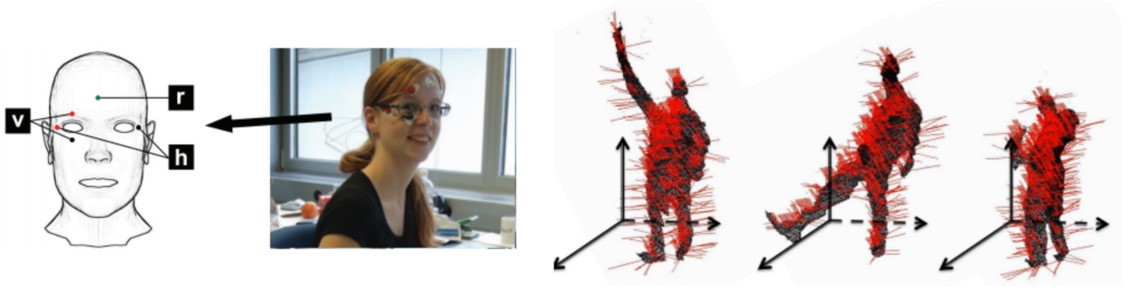
\includegraphics[width=0.8\textwidth]{images/rel_app_activity}
\caption{\emph{Left:} Eye movement tracker by Bulling \cite{bulling2011eye}. \emph{Right:} Hon4D - surface normals of different activities \cite{oreifej2013hon4d}}
\label{fig:rel_app_activity}
\end{figure}	

When trying to determine human activities wearable sensors are an important approach that has been used extensively. It is possible to use either physiological measurements or movement data. A classic work in this domain presented by Bao et al. is associating activities based on movement data generated by accelerometers \cite{Bao2004}. This sensor category is able to detect the acceleration in multiple directions, e.g. commonly used to detect the orientation of mobile devices. Using five different sensors attached to arms, legs and hip, they were able to associate 20 different activities performed by 20 different subjects with an accuracy of approximately $80\%$.

In some application domains that have a specific set of tasks other approaches might be suitable. An interesting system was presented by Bulling et al. that tries to determine activities based on the movement of the eyes \cite{bulling2011eye}. They are attaching a set of electrodes to the user's head to track the activity of muscles around the eye, without using any external sensors such as gaze trackers. The setup and electrode placing is shown in Figure \ref{fig:rel_app_activity} on the left. In a study with eight users they tried to distinguish five different typical office work activities using SVM classification. These activities are copying text between documents in a two monitor setup, reading a document on the table, writing on a page on the table, watching a video and browsing the internet. The achieved average precision was $76\%$ and recall $71\%$.

A common problem in situation classification is labeling of the acquired data to a given situation. Typically this is performed manually by the researcher. Lasecki et al. introduced Legion:AR, a system that allows to crowdsource this process to a large group of workers that individually label activities from a video feed \cite{lasecki2013real}. They could show that while in complex situations a group of five persons labeled $90\%$ of activities and objects correctly, while a single person only reaches $48\%$ on average. The process is aided by integrating the input from different persons that are currently labeling.

A final example in the domain of activity recognition is Hon4D, a system that infers situation from depth camera sequences \cite{oreifej2013hon4d}. They suggest the histogram of normal orientation in depth, time and spatial coordinates as a feature for activities from depth data. Examples of surface normals for different activities and body surfaces are shown in Figure \ref{fig:rel_app_activity} on the right. The advantage of this operator is that it takes into account the movement of the overall surface of recognized persons, as opposed to silhouettes or the reconstructed skeleton joints. This approach reaches classification precision between $89\%$ and $97\%$ when used on common activity depth data sets. 

\subsection{Smart appliances}
Smart appliances are devices that are attentive to their environment \cite{schmidt2001build}. This is usually achieved by integrating different sensors and actuators to provide additional functions and services to a user. Some examples include intelligent furniture that can detect their occupation, internet-connected household items, or single-purpose devices, e.g. providing reminder services. An overview of different examples can be found by Park et al. \cite{park2003smart}. 

\begin{figure}[ht]
\centering
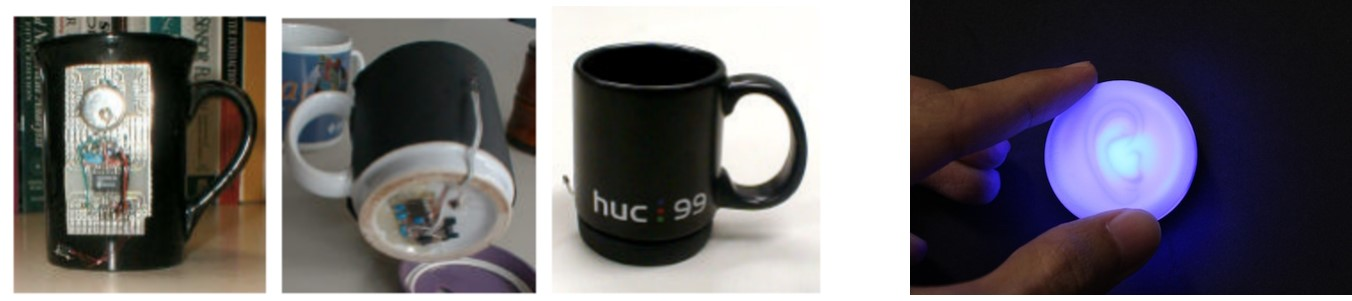
\includegraphics[width=0.8\textwidth]{images/rel_app_appliances}
\caption{\emph{Left:} Different MediaCup prototype \cite{gellersen1999mediacup}. \emph{Right:} Stickear system to augment appliances with audio sensing \cite{yeo2013stickear}}
\label{fig:rel_app_appliances}
\end{figure}	

One example for common household items augmented with additional features is the MediaCup by Gellersen et al. \cite{gellersen1999mediacup}. This coffee cup is augmented with temperature and acceleration sensors, a processing unit and communication using an infrared system. Some of the prototypes are shown in Figure \ref{fig:rel_app_appliances} on the left. It is able to sense if there is fresh coffee in the cup, if it currently used for drinking, stationary or being played with. The applications were focused on remote colleague awareness, whereas the activities of the MediaCup were transmitted to a remote location.

StickEar by Yeo et al. is a wireless device that adds different capabilities to objects it is attached to \cite{yeo2013stickear}. They integrate a rotary switch, buttons, microphone, speaker and processing and communication components into a small portable package, as shown in Figure \ref{fig:rel_app_appliances} on the right. Some supported interactions are control of devices using sound, autonomous response to sound events, or remote triggering of sound. The system can be controlled using an app for mobile devices.

There is a number of smart appliances in the medical domain. They try to provide different services related to health and well-being. A common example are smart medication dispensers, such as the one presented by Tsai et al. \cite{tsai2011smart}. Based on a medication schedule it will dispense the right medication and dose at the specified times. They include a few different algorithms for heuristic scheduling based on a collaborative approach between scheduler and the controller of the dispenser.

When deploying smart appliances it is necessary to provide energy to the systems. If there is no socket nearby batteries or other methods have to be used. If the system is capable to independently harvest the energy from environment sources. One example are the bistable display tags by Dementyev et al. \cite{dementyev2013wirelessly}. They rely on e-paper displays that keep their screen content unless a refresh is triggered. Using an energy harvesting IC it is possible to transfer enough information and the new screen content via NFC. In an example application screenshots from a smartphone could be transferred to the display.

\subsection{Mobile devices}
In his famous article, Mark Weiser coined three different forms of devices - tags, tabs and boards \cite{Weiser1991}. They are primary distinguished by their size and how they can be used for interaction with the system. The prevalet smart phones and tablets nowadays resemble closely the envisioned smart tab - handheld devices that provide sensing, interaction and communication facilities supported by sufficient processing power. Consequently, they are used very often in smart environment applications.

\begin{figure}[ht]
\centering
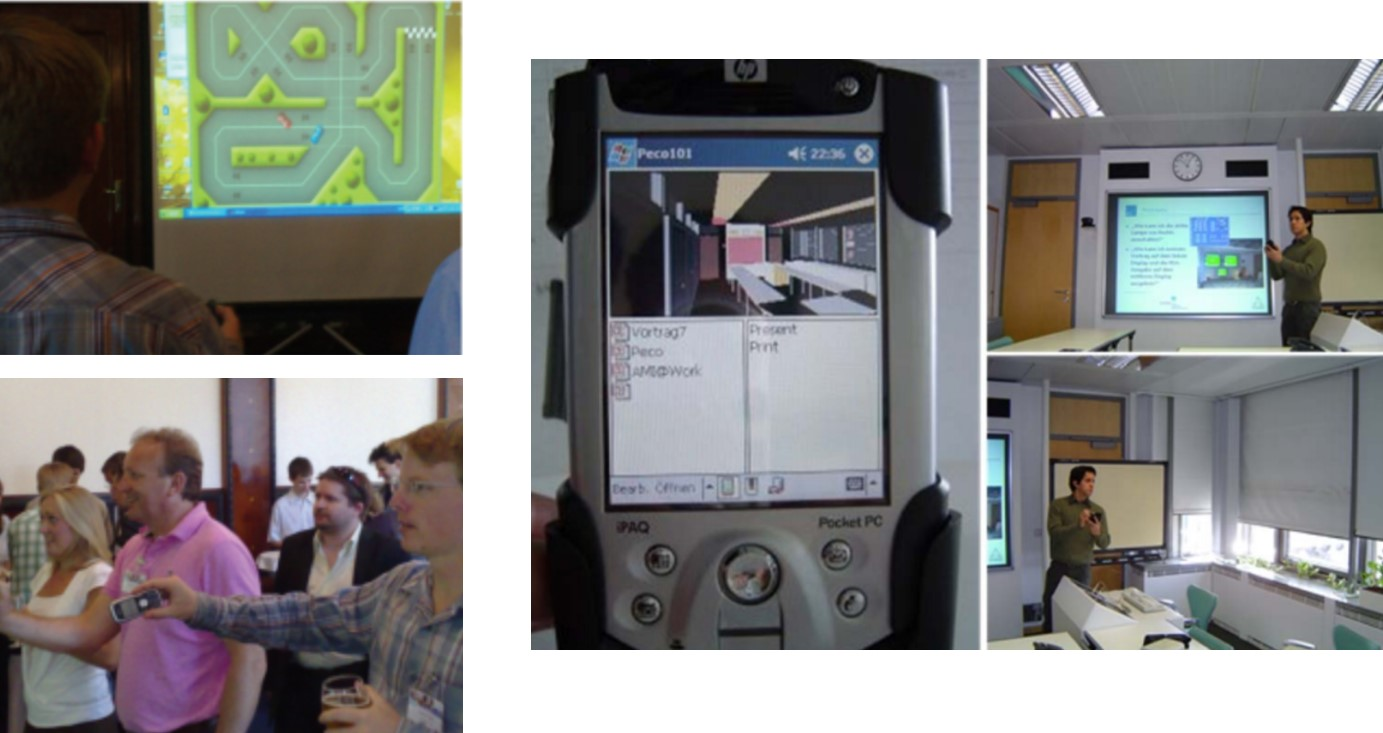
\includegraphics[width=0.8\textwidth]{images/rel_app_mobile}
\caption{\emph{Left:} TiltRacer controlled by accelerometers of mobile phones \cite{vajk2007using}. \emph{Right:} PECo environment control application on a PDA \cite{shirehjini2004novel}}
\label{fig:rel_app_mobile}
\end{figure}

Ballages et al. collected and investigated numerous ways how smart phones can be used to in ubiquitous computing \cite{ballagas2006smart}. They provided an overview of different positioning, orientation and selection methods, including using the camera on the mobile phone and different processing methods to control a cursor. An important contribution was a classification of potential mobile phone interactions and a summary of of position, orientation and selection techniques.

Bluetone is a system created by Dearman and Truong that allows to control public displays using mobile phones via Bluetooth communication \cite{dearman2009bluetone}. In order to avoid installing any additional application they are using the Bluetooth headset profile and transfer sounds instead of packaged information. Similarly Vajk et al. proposed using the accelerometers in a phone to control applications on a large public display \cite{vajk2007using}. One example application was TiltRacer that could be controlled by different users standing in front of a display, as shown in Figure \ref{fig:rel_app_mobile} on the left.

Nazari Shirejini presented PECo, an environment controller based on a PDA device \cite{shirehjini2004novel}. Based on a 3D model of the current environment it was possible to control different appliances by selecting them on the mobile device. Additionally, a concept was presented that allows to transfer documents from the PDA to different suitable devices, by using simple drag \& drop operations. The practical use case was implemented in a lecture room and connected to the controlling system, e.g. allowing to display documents on a projector by dropping them on the 3D model of the projecting screen. The system is shown in Figure \ref{fig:rel_app_mobile} on the right.

A final example is in the popular domain of augmented reality systems for mobile devices. There are numerous popular applications that overlay additional information on a live camera image of mobile phones. Olsson et al. tried to evaluate user experience and acceptance of different mobile augmented reality applications \cite{olsson2012user}. They found that information applications were better received than entertainment applications. In addition, information flood, loss of autonomy and virtual replacement of actual items were seen as most negative aspects of this technology.


\subsection{Autonomous systems}
Autonomous systems are an important future application in smart environments. While factory complexes started using robots decades ago, the trend towards home robotics is fairly recent, as the processing and sensing capabilities of the systems increased, while the price could be reduced significantly. There are numerous potential use cases, ranging from vacuuming or gardening robots, to full-service robots that can be used in care systems for the elderly. In this section I will present four different examples, how autonomous systems can be used in smart environments.

\begin{figure}[ht]
\centering
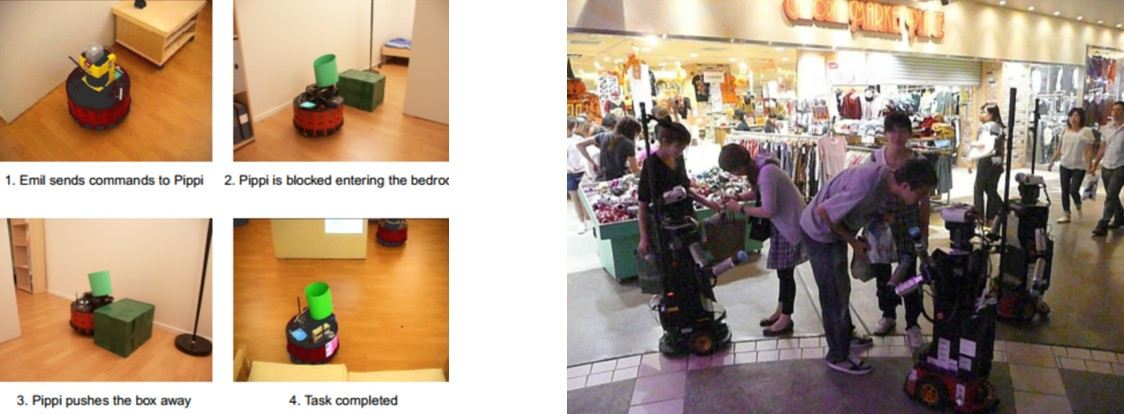
\includegraphics[width=0.8\textwidth]{images/rel_app_robots}
\caption{\emph{Left:} Scenario of the PEIS system \cite{broxvall2006peis}. \emph{Right:} Robots moving around in a social environment \cite{glas2009simultaneous}}
\label{fig:rel_app_robots}
\end{figure}

Coradschi and Saffiotti propagated the symbiotic properties of robots operating in a smart environment \cite{coradeschi2006symbiotic}. Human, robot and smart environment are modeled as three distinct actors that share resources and information between each other. The distributed systems in the environment, e.g. sensors, tags and actuators, can deliver additional information to the control unit of the autonomous system that can be used to optimize any strategies. Similarly, users can benefit from the coordination between robot and environment to achieve common goals.

An implementation of a similar concept was published by Broxvall et al. \cite{broxvall2006peis}. PEIS, a network of heterogeneous smart devices that operate in a smart environment. In the example scenario shown in Figure \ref{fig:rel_app_robots} on the left. A coordinating system (Emil) sends commands to a robot (Pippi) that moves around the house but has his path blocked by a parcel. As this parcel is a smart object and knows its contents this information is forwarded to the robot, who then safely moves the parcel away. Thus, a collaboration between smart environments and robots can support similar scenarios that reduces the requirements for both environments and robots.

Glas et al. investigated how robots can track people and localize themselves in social environments, that are frequented by a larger number of persons \cite{glas2009simultaneous}. They combine laser range-scanners placed in the environment that provide wide coverage and are able to track the trajectories of moving persons and robots. This is combined using Kalman filtering with the odometry data generated by the robots. As a combined solution this enables localization of both people and robots in a shared global coordinate system. One example application system is shown in Figure \ref{fig:rel_app_robots} on the right, whereas robots provide directional information to shoppers in a mall.

A final example that evaluates user experiences gathered in different research projects was presented by Huijnen et al.  \cite{huijnen2011maybe}. Within the projects CompanionAble and Mobiserv different service robots were deployed in smart home environments for elderly persons. The user trials involved testing interaction and usability, user acceptance and privacy. The robots user - Hector and Kompai - are designed to provide assistance for persons with Mild Cognitive Impairments or early stages of dementia. One result was that the appearance of the robot was not particularly important for this user group, as opposed to the functionality, which was considered most important. 
